\section{Modelo de información del sistema}
En la Figura \ref{fig:Base_ServidorEmbebido} se observa un diagrama del modelo de información correspondiente al servidor embebido, se puede observar que las tablas no se encuentran relacionadas, esto es debido a que la información que almacenan no está ligada de ninguna forma con el resto, a pesar de que los registros de algunas tablas sirvan para calcular los registros de otras, cada tabla representa un archivo JSON, que a su vez representa un arreglo de objetos con los atributos como se especifica en la figura \ref{fig:Base_ServidorEmbebido}, en la muestra de tiempo real se guarda el valor actual segundo a segundo del un nodo del sensor, en las muestras del día, se almacenarán un total de 120 objetos definidos por el horario de muestreo, en las muestras del mes, los promedios de los 28, 30 ó 31 días del mes y en el de muestras del año muestras del año los 12 promedios de cada mes del año.

\begin{figure}[H]
	\centering
	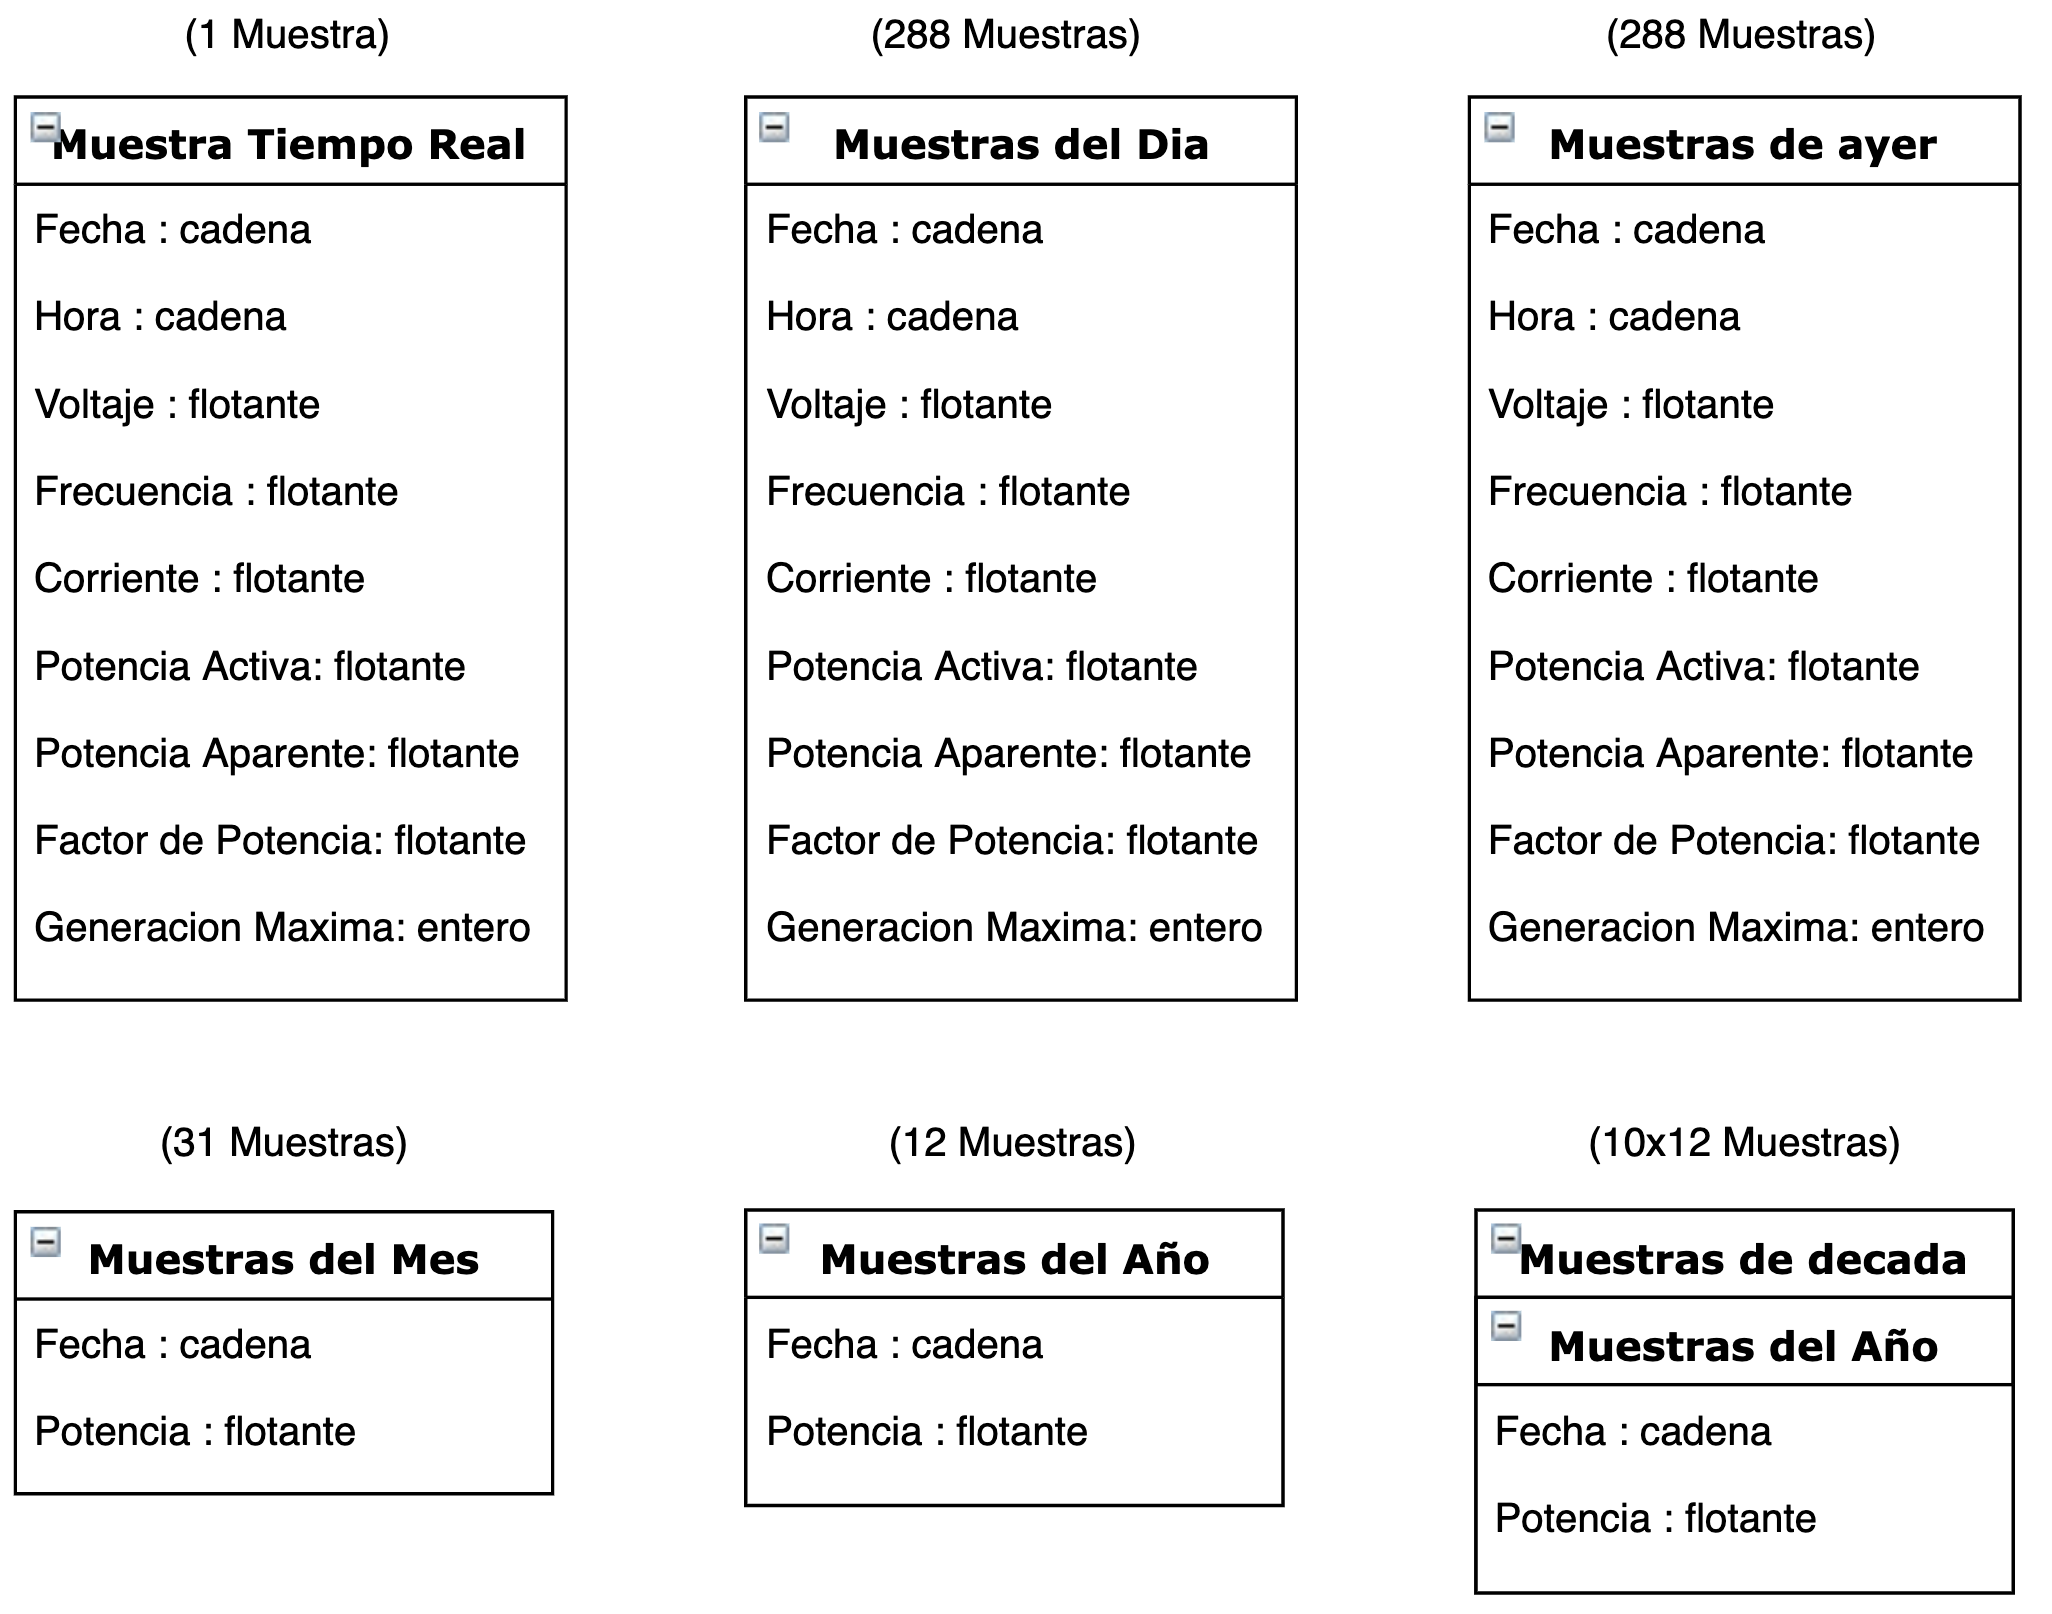
\includegraphics[scale=.35]{Capitulo4/images/Base_ServidorEmbebido.png}
	\caption{Modelo de información del Servidor Embebido}
	\label{fig:Base_ServidorEmbebido}
\end{figure}

A continuación en la Figura \ref{fig:Base_AplicacionUsuario} se muestra el diagrama del modelo de información correspondiente a la aplicación de usuario, en donde se puede observar que únicamente se almacenará en la aplicación las notificaciones y los servidores que den respuesta a las peticiones de la aplicación de usuario, la relación entre tablas nos indica que muchas notificaciones pueden pertenecer a un mismo servidor.

\begin{figure}[H]
	\centering
	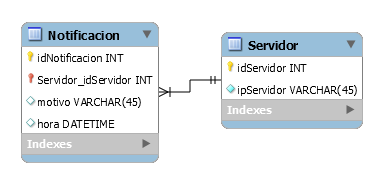
\includegraphics[scale=1]{Capitulo4/images/Base_AplicacionUsuario.PNG}
	\caption{Modelo de información de la aplicación de usuario}
	\label{fig:Base_AplicacionUsuario}
\end{figure}